\documentclass{book}

\usepackage{graphicx}
\usepackage{multicol}
%\usepackage{multirow}
%\usepackage{bm} %% bold face math symbols
\usepackage{listings}
\usepackage{../macros/mytikz}
\usetikzlibrary{shapes}
%\usepackage{stmaryrd}%\newcommand{\contra}{\lightning}
%\usepackage{rotating} \newcommand{\sw}[1]{\begin{sideways}#1\end{sideways}}

\usepackage{../macros/algorithm}
%\usepackage{ded}
\usepackage{../mylecturenotes}
\usepackage{../macros}

\title{Lectures Notes on Secure and Dependable Systems}
\author{Florian Rabe}
\date{2017}


\begin{document}
\maketitle

\tableofcontents
\newpage

\part{Introduction}

 \chapter{Meta-Remarks}
  \begin{center}
\textbf{Important stuff that you should read carefully!}
\end{center}

\paragraph{State of these notes}
I constantly work on my lecture notes.
Therefore, keep in mind that:
\begin{compactitem}
\item I am developing these notes in parallel with the lecture --- they can grow or change throughout the semester.
\item These notes are neither a subset nor a superset of the material discussed in the lecture. On the one handle, they may contain more details than mentioned in the lectures. On the other hand, important material such as background, diagrams, and examples may be part of the lecture but not mentioned in these notes.
\item Unless mentioned otherwise, all material in these notes is exam-relevant (in addition to all material discussed in the lectures).
\end{compactitem}
\medskip

\paragraph{Collaboration on these notes}
I am writing these notes using LaTeX and storing them in a git repository on GitHub at \url{https://github.com/florian-rabe/Teaching}.
As an experiment in teaching, I am inviting all of you to collaborate on these lecture notes with me.
This would require familiarity with LaTeX as well as Git and GitHub --- that is not part of this lecture, but it is an essential skill for you.
Ask in the lecture if you have difficulty figuring it out on your own.
\medskip

By forking and by submitting pull requests for this repository, you can suggest changes to these notes.
For example, you are encouraged to:
\begin{compactitem}
\item Fix typos and other errors.
\item Add examples and diagrams that I develop on the board during lectures.
\item Add solutions for the homeworks if I did not provide any (of course, I will only integrate solutions after the deadline).
\item Add additional examples, exercises, or explanations that you came up or found in other sources.
 If you use material from other sources (e.g., by copying an diagram from some website), make sure that you have the license to use it and that you acknowledge sources appropriately!
\end{compactitem}
I will review and approve or reject the changes.
If you make substantial contributions, I will list you as a contributor (i.e., something you can put in your CV).
\medskip

Any improvement you make will not only help your fellow students, it will also increase your own understanding of the material.
%Therefore, I can give you up to $10\%$ bonus credit for such contributions.
Make sure your git commits carry a user name that I can connect to you.)

\paragraph{Other Advice}
I maintain a list of useful advice for students at \url{https://github.com/florian-rabe/Teaching/blob/master/general/advice_for_students.pdf}.
It is mostly targeted at older students who work in individual projects with me (e.g., students who work on their BSc thesis).
But much of it is useful for you already now or will become useful soon.
So have a look.

  \chapter{Concepts}
   \section{Abbreviations}

\begin{center}
\begin{tabular}{lll}
knowledge representation and processing & KRP & the general area of this course \\
knowledge representation language & KRL & a languages used in KRP \\
knowledge representation tool & KRT & a tool implementing a KPL and processing algorithms for it
\end{tabular}
\end{center}

\section{Motivation}

\subsection{Knowledge}

Human knowledge pervades all sciences including computer science, mathematics, natural sciences and engineering.
That is not surprising: ``science'' is derived from the Latin word ``scire'' meaning ``to know''.
Similarly, philosophy, from which all sciences derive, is named after the Greek words ``philo'' meaning loving and ``sophia'' meaning wisdom, and the for common ending ``-logy'' is derived from Greek ``logos'' meaning word (i.e., a representation of knowledge).

In regards to knowledge, computer science is special in two ways:
Firstly, many branches of computer science need to understand KRP as a prerequisite for teaching computers to do knowledge-based tasks.
In some sense, KRP is the foundation and ultimate goal of all artificial intelligence.%
\footnote{Indeed, a major problem with the currently very successful machine learning-based AI technology is that it remains unclear when and how it does KRP. That can be dangerous because it leads to AI systems recommending decisions without being able to explain why that decision should be trusted.}
Secondly, modern information technology enables all sciences to apply computer-based KRP in order to vastly expand on the domain-specific tasks that can be automated.
Currently all sciences are becoming more and more computerized, but most non-CS scientists (and many computer scientists for that matter) lack a systematic education and understanding of IT-KRP.
That often leads to bad solutions when domain experts cannot see which KRP solutions are applicable or how to apply them.

\subsection{Representation and Processing}

It is no coincidence that this course uses the phrase ``Representation and Processing''.
In fact, this is an instance of a universal duality.
Consider the following table of analogous concept pairs, which could be extended with many more examples:

\begin{center}
\begin{tabular}{l|l}
Representation & Processing \\
\hline
Static & Dynamic \\
Situation & Change \\
Be & Become \\
Data Structures & Algorithms \\
Set & Function \\
State & Transition \\
Space & Time
\end{tabular}
\end{center}

Again and again, we distinguish a static concept that describes/represents what is a situation/state is and a dynamic concept that describes how it changes.
If that change is a computer doing something with or acting on that representation, we speak of ``processing''.

It is particular illuminating to contrast KRP to the standard CS course on Data Structures and Algorithms (DA).%
\footnote{The course is typically called ``Algorithms and Data Structures'', but that is arguably awkward because algorithms can exist if there are data structure to work with. Compare my notes on that course in this repository, where I emphasize data structures much more than is commonly done in that course.}
Generally speaking, DA teaches the methods, and KRP teaches how to apply them.
Data structures are a critical prerequisite for representing knowledge.
But data structures alone do not capture what the data means (i.e., the knowledge) or if a particular representation makes any sense.
Similarly, algorithms are the critical prerequisite for processing knowledge.
But while algorithms can be systematically analyzed for efficiency, it is much harder to analyze if an algorithm processes knowledge correctly.
The latter requires understanding what the input and output data means.

Capturing knowledge in computers is much harder than developing data structures and algorithms.
It is ultimately the same challenge as figuring out if a computer system is working correctly --- a problem that is well-known to be undecidable in general and very difficult in each individual case.

%%%%%%%%%%%%%%%%%%%%%%%%%%%%%%%%%%%%%%%%%%%%%%%%%%%%%%%%%%%%%%%
\section{Components of Knowledge}

\subsection{Syntax and Semantics, Data and Knowledge}

Four concepts are of particular relevance to understanding knowledge.
They form a $2\times 2$-quadruple of concepts:

\begin{center}
\begin{tabular}{l|l}
Syntax & Data \\
\hline
Semantics & Knowledge
\end{tabular}
\end{center}

All four concepts are primitive, i.e., they cannot be defined in simpler terms.
All sciences have few carefully-chosen primitive on which everything builds.
This is done most systematically in mathematics (where primitives include set or function).
While mathematical primitives as well as some primitives in physics or CS are specified formally, the above four concepts can only be described informally, ultimately appealing to pre-existing human understanding.
Moreover, this description is not standardized --- different courses may use very different descriptions even they ultimately try to capture the same elusive ideas.

\textbf{Data} (in the narrow sense of computer science) is any object that can be stored in a computer, typically combined with the ability to input/output, transfer, and change the object.
This includes bits, strings, numbers, files, etc.

Data by itself is useless because we would have no idea what to do with it.
For example, the object $O=((49.5739143, 11.0264941), "2020-04-21T16:15:00CEST")$ is useless data without additional information about its syntax and semantics.
Similarly, a file is useless data unless we know which file format it uses.

\textbf{Syntax} is a system of rules that describes which data is \textbf{well-formed}.
For $O$ above the syntax could be ``a pair of (a pair of two IEEE double precision floating point numbers) and a string encoding of an time stamp''. 
For a file, the syntax is often indicated by the file name extension, e.g., the syntax of an \texttt{html} file is given in Section 12 of the current HTML standard\footnote{\url{https://html.spec.whatwg.org/multipage/}}.

Syntax alone is useless unless we know what the semantics, i.e., what the data means and thus how to correctly interpret and process the data.
For example, the syntax of $O$ allows to check that $O$ is well-formed, i.e., indeed contains two numbers and a timestamp string.
That allows rejecting ill-formed data such as $((49.5739143, 11.0264941), "foo")$.
The HTML syntax allows us to check that a file conforms to the standard.

\textbf{Semantics} is a system of rules that determines the meaning of well-formed data.
For example, ISO 8601 specifies that timestamp string refer to a particular date and time in a particular time zone.
Further semantics for $O$ might be implicit in the algorithms that produce and consume it: such as ``the first component of the pair contains two numbers between $0$ and $180$ resp. $0$ and $360$ indicating latitude resp. longitude of a location on earth''.
Semantics might be multi-staged, and further semantics about $O$ might be that $O$ indicates the location and time of the first lecture of this course.
Similarly, Section 14 of the HTML standard specifies the semantics of well-formed HTML files by describing how they are to be rendered in a web browser.

\textbf{Knowledge} is the combining of some data with its syntax and semantics.
That allows applying the semantics to obtain the meaning of the data (if syntactically well-formed and signaling an error otherwise).
In computer systems,
\begin{compactitem}
 \item data is represented using primitive data (ultimately the bits provided by the hardware) and encodings of more complex data (bytes, arrays, strings, etc.) in terms of simpler ones,
 \item syntax is theoretically specified using grammars and practically implemented in programming languages using data structures,
 \item semantics is represented using algorithms that process syntactically well-formed data,
 \item knowledge is elusive and often emerges from executing the semantics, e.g., rendering of an HTML file.
\end{compactitem}

\subsection{Semantics as Syntax Transformation}

In order to capture knowledge better in computer systems, we often use two syntax levels: one to represent the data itself and another to represent the knowledge.
These can be seen as input and output data.
In that case, semantics is a function that translates from the data syntax to the knowledge syntax, and knowledge is the pair of the data and the result of applying the semantics.
The following table gives some examples.

\begin{center}
\begin{tabular}{l|l|l}
Data syntax & Semantics function & Knowledge syntax \\
\hline
SPARQL query & evaluation & result set \\
SQL query & evaluation & result table \\
program & compiler & binary code \\
program expression & interpreter & result value \\ 
logical formula & interpretation in a model & mathematical object \\
HTML document & rendering & graphical representation 
\end{tabular}
\end{center}

Thus, the role of syntax vs. semantics may depend on the context: just like one function's output can be another function's input, one interpretation's knowledge can be another one's syntax.
For example, we can first compile a program into binary and then execute it to returns its value.

Such hierarchies of evaluation levels are very common in computer systems.
In fact, most state-of-the-art compilers are subdivided into multiple phases each further interpreting the output of the previous one.
Thus, if knowledge is represented in computers, it is invariably data itself but relative to a different syntax.

\subsection{Heterogeneity of Semantics and Knowledge}

While it is easy to design languages to represent data in general, it is very difficult to designing KRLs that capture the human-level quality of knowledge.
Over the last few decades, the KRP area in computer science has diversified into different subareas that approach this research problem in fundamentally different ways.
In fact, KRP in the very general sense of this course is usually not even studied by itself --- instead the subareas are so different, specialized, and large that they all sustain their respective university courses and research conferences.

This is related to the fact the data naturally comes in fundamentally different forms such as graphs, arrays, tables in the sense of relational databases, programs in a programming language, logical formulas, or natural language texts.
We speak of \textbf{heterogeneous} data.
These different forms of data are supported by highly specialized KPTs: graph databases, array databases, relational databases, package databases for programming languages, theorem databases for logics (e.g., the Isabelle Archive of Formal Proofs), databases of research papers (such as the arXiv), and so on.

All of these are very successful for their respective kind of data.
And all of them include specifications of semantics and KP algorithms that implement this semantics.
But it can very massively how the semantics is specified and implemented.
This has cause major practical problems for tool interoperability: many projects require data in multiple formats and algorithms from multiple tools.
But the respective tools are often islands that assume that all data is represented in the tool's language and users do not use outside tools.
Therefore, the import/export capabilities of the tools are often limited.

Moreover, transporting data across systems is usually ignorant of the semantics: while each tool takes relatively good care to implement the semantics correctly, there is much less certainty that the semantics is preserved when exchanging data across tools.
For a trivial example, consider a tool that measure length in inches vs. a tool that uses centimeters, both using floating point numbers for the data: if they exchange the data, i.e., just the numbers, they may mis-communicate the semantics.%
\footnote{Problems like this have been involved in major disasters such as the Mars Climate Orbiter.} 

This problem is not easy to fix though.
The heterogeneity of data and semantics is so extreme that it is, in some cases, an open theoretical problem how knowledge can be shared at all across tools.
The basic idea --- exchange the data in a way that preserves semantics --- can be difficult to implement if both tools use entirely different paradigms to specify semantics.

%%%%%%%%%%%%%%%%%%%%%%%%%%%%%%%%%%%%%%%%%%%%%%%%%%%%%%%%%%%%%%%
\section{The Tetrapod Model of Knowledge}

The Tetrapod model of knowledge is an ongoing research project by the instructors of this course.
A first publication was made in \cite{CFKR:tetrapod:19}.
The structure of this course will draw heavily on the Tetrapod model to get an overview of the different approaches to KPR and their interoperability problems.

\subsection{Five Aspects of Knowledge}

The Tetrapod model distinguishes five basic \textbf{aspects} of knowledge and KPR as described below.
For each aspect, there is a variety dedicated KRLs supported by highly optimized KPTs as indicated in the following table:

\begin{center}
\begin{tabular}{lll}
Aspect & KRLs (examples) & KPTs (examples) \\
\hline
ontologization & ontology languages (OWL), description logics (ALC) & reasoners, SPARQL engines (Virtuoso) \\
concretization & relational databases (SQL, JSON) & databases (MySQL, MongoDb) \\
computation & programming languages (C) & interpreters, compilers (gcc) \\
deduction & logics (HOL) & theorem provers (Isabelle) \\
narration & document languages (HTML, LaTeX) & editors, viewers
\end{tabular}
\end{center}

\textbf{Ontologization} focuses on developing and curating a coherent and comprehensive ontology of concepts.
This focuses on identifying the central concepts in a domain and their relations.
For example, a medical ontology would define concepts for every symptom, disease, and medication and then define relations for which symptoms and medications are related to which disease.

Ontologies typically abstract from the knowledge: they standardize identifiers for the concepts and spell out some properties and relations but do not try to capture all details of the knowledge.
Well-designed ontologies can capture exactly that different KPTs must share and can thus serve as interoperability layers between them.

While organization can use ontology languages such as OWL or RDF, the inherent complexity of formal objects in computer science and mathematics usually requires going beyond general purpose ontology languages (similar to how the programming languages underlying computer algebra systems usually go beyond general purpose programming languages).

\textbf{Concretization} uses languages based on numbers, strings, lists, and records to obtain concrete representations of datasets in order to store and query their properties efficiently.
Because concrete objects are so simple and widely used, it is possible and common to build concrete datasets on top of general purpose data representation languages and tools such as JSON or SQL.

\textbf{Computation} uses specification and programming languages to represent algorithmic knowledge.

\textbf{Deduction} uses logics and theorem provers  to obtain verifiable correctness.

\textbf{Narration} uses natural language to obtain texts are easy to understand for humans.
Because narrative languages are not well-standardized (apart from general purpose languages such as free text or \LaTeX), it is common to develop narrative libraries on top of ad-hoc languages that impose some formal structure on top of informal text, such as a fixed tree structure whose leafs are free text or a particular set of {\LaTeX} macros that must be used.
Narrative libraries can be classified based on whether entries are derived from publications (e.g., one abstract per paper in zbMATH) or mathematical concepts (e.g., one page per concept in $n$Lab).
%While these languages have multiple implementations, individual libraries usually involve specific encodings that are implemented only by a single tool.

%For example, an organization language might state only a function's type and properties.
%A computational treatment provides an efficient implementation, a deductive one proves the properties, a concretized one tables the function's values, and a narrative one documents the nature and purpose of the function.


\subsection{Relations between the Aspects}

The aspects can be visualized as the corners of tetrahedron with ontologization in the center and edges and faces representing solutions that mix two or three aspects as seen in Figure~\ref{fig:tetrapod}.

\begin{figure}[hbt]
\begin{center}
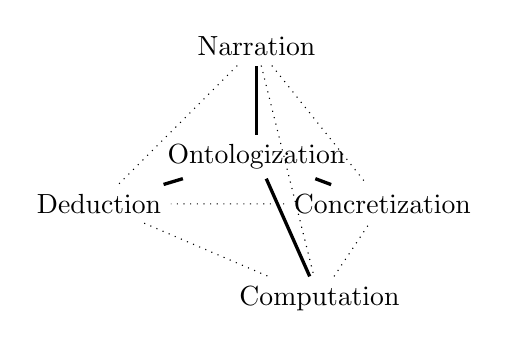
\begin{tikzpicture}[scale=4]
  \node (center) at (0,.15) {Ontologization};
  \node (left) at (.2,-.3) {Computation};
  \node (right) at (.4,0) {Concretization};
  \node (back) at (-.5,0) {Deduction};
  \node (up) at (0,.5) {Narration};

  \draw[very thick] (center) -- (left);
  \draw[very thick] (center) -- (right);
  \draw[very thick] (center) -- (back);
  \draw[very thick] (center) -- (up);
  \draw[dotted] (left) -- (right) -- (back) -- (left);
  \draw[dotted] (up) -- (left);
  \draw[dotted] (up) -- (right);
  \draw[dotted] (up) -- (back);
\end{tikzpicture}
\end{center}
\caption{Tetrapod model of knowledge}\label{fig:tetrapod}
\end{figure}

\begin{figure}[htb]\centering\footnotesize\setlength{\tabcolsep}{4pt}
\begin{tabular}{|l|llp{2.1cm}l|}\hline
       & \multicolumn{4}{c|}{characteristic} \\
Aspect &  objects & advantage & joint advantage of the other aspects & application \\\hline
deduction & formal proofs & correctness & ease of use & verification \\
computation & programs & efficiency & well-definedness & execution\\
concretization & concrete objects & tangibility & abstraction & storage/retrieval\\
narration & texts & flexibility & formal semantics & human understanding\\\hline
\end{tabular}
\quad
\begin{tabular}{|l|l|}\hline
Aspect pair & characteristic advantage \\\hline
ded./comp.  & rich meta-theory \\
narr./conc. & simple languages \\\hline
ded./narr.  & theorems and proofs \\
comp./conc. & normalization \\\hline
ded./conc.  & decidable well-definedness \\
comp./narr. & Turing completeness \\\hline
\end{tabular}
\caption{Shared properties and advantages of aspects}\label{fig:tetrapod2}
\end{figure}

Most approaches try to incorporate all or multiple aspects.
But all languages and tools tend to be heavily biased towards and optimized for a single one of the four corner aspects.
This is not due to ignorance but because each aspect provides characteristic advantages that are extremely hard to capture at once.
In fact, every combination of aspects shares characteristic advantages and disadvantages as sketched in Figure~\ref{fig:tetrapod2}.
For example, deductive and narrative definitions of a function involved well-definedness arguments, and a function defined by a concrete table is trivially well-defined, but a computational definition of a function may throw exceptions when running; but only the latter can store and compute functions efficiently.
Consequently, dedicated and mostly disjoint communities have evolved that have produced large aspect-specific datasets.

%\subsection{Aspect-Specific Datasets in Mathematics}
%
%A survey of the state of the art in aspects is huge.
%Figure~\ref{fig:libraries} gives an overview of important datasets just the domain of mathematics.
%We have also pre-published a draft of an extensive survey in \cite{CarFarSharBerKohMueRab:somss20}.
%
%Crucially, these disjoint projects overlap massively.
%For example, the concept of \emph{group} is defined in most proof assistants and computer algebra systems, concrete groups are part of multiple large libraries (e.g., as the main object of interest in the small groups libraries, or as symmetry groups arising from other objects), and has entries in most narrative libraries (e.g., with entries in Stacks and nLab).
%Despite the overwhelming practical need, at the moment there is little to no technology to integrate libraries across this overlap.
%The same effect is found in other domains.
%
%\begin{figure}[ht]\centering\small\def\cite#1{}
%  \begin{tabular}{| p{.3\textwidth} | p{0.55\textwidth}|}\hline
%  Dataset & Description and approximate size \\\hline\hline
%  \multicolumn{2}{|l|}{\textbf{Inference}} \\\hline
%  Theorem prover libraries  & ??? \\\hline
%  \multicolumn{2}{|l|}{\textbf{Computation} \hfill\strut\hfill {\tiny CAS = computer algebra system}} \\\hline
%  Mathematica & commercial CAS, $5k$ built-in functions, $150$k official examples\\\hline
%  Maple & commercial CAS, $5$k built-in functions \\\hline
%  GAP \cite{gap} & CAS for group theory, $10$k statements \\\hline
%  Singular \cite{singular:on} & CAS for polynomials, over $90$ libraries \\\hline
%  SageMath \cite{SageMath:on} & $1$k modules, bundled with $4$GB of CAS tools and libraries\\\hline
%  Modelica \cite{Modelica:on} & modeling language, $5$k built-in classes, $100$ open source libraries, $50$ commercial libraries up to $0.5$M equations \\\hline\hline % $10$ official, $>100$ open-source, $50$ commercial,
%  \multicolumn{2}{|l|}{\textbf{Concretization}} \\\hline
% OEIS \cite{OEIS:on} & $330$k integer sequences, $1$ TB; $0.3$M sequence identities in \cite{kwarc:datahost:on} \\\hline
%%  OEIS identities \cite{kwarc:datahost:on} & $0.3$M sequence identities, $2.5$ TB \\\hline
% various databases of graphs\cite{ConderCensuses:on, HartleyPolytopes:on, LeemansPolytopes:on, PotocnikCensuses:on, RoyleVT:on, WilsonET:on} & highly symmetric graphs, maps, polytopes, $30$ datasets, $2$M objects, $1$TB \\\hline
%  various databases of lattices \cite{KohLat:on, LeeLat:on, MalLat:on} & $7$ datasets, $17$G objects, $1.5$ TB \\\hline
%  findstat \cite{findstat} & combinatorial statistics and maps, $1.5$k objects \\\hline
%  SageMath databases \cite{SageDB:on} & $12$ datasets \\\hline
%  $L$-functions and modular forms \cite{lmfdb:on} & $80$ datasets, $1$G objects, $1$ TB \\\hline
%  Small Groups Library \cite{BeEiOBSmallGroups} & $450$M groups, $80$ MB \\\hline\hline
%  \multicolumn{2}{|l|}{\textbf{Narration}\hfill\strut\hfill {\tiny based on publications (P) or concepts (C)}} \\\hline
%  arXiv.org (P) & $300$k math preprints, most with {\LaTeX} sources\\\hline
%  zbMATH \cite{zbMATH:on} (P) & $4$M publication abstracts with semantic data, $30$M reference data, $1$M disambig. authors, $2.7$M full text links \\\hline % $1$M OA 
%  EuDML  \cite{EuDML:on} (P) & $260$k open full-text publications, digitized journal back issues \\\hline
%%  MathOverFlow & $\approx 1,1$M questions/answers, $\geq11$K answer authors \\\hline
%  Stacks project (C) & $6$k pages, semantically annotated, curated, searchable textbook \\\hline
%  $n$Lab (C) & $13$k pages on category theory and applications\\\hline
%  SMGloM glossary (C) & $1$k modules, $2$k concepts, $4.5$k multi-lingual verbalizations in English \\\hline\hline %  (100\%), German (90\%), Chinese (10\%)
%  \multicolumn{2}{|l|}{\textbf{Organization}} \\\hline
%  swMATH \cite{swMATH:on} & $25$k software records with $300$k links to $180$k publications \\\hline
%  Wikidata  \cite{wikidata:on} & $34$GB linked data, $4$k formulas, interlinked with named theorems, persons, publications \\\hline
%  DLMF & $500$ special mathematical functions, $10$k formulas \\\hline
%  OpenMath CDs \cite{openmath} & curated reference points for $1.5$k concepts \\\hline
%  LATIN atlas \cite{CHKMR:latinabs:11,LATIN:online} & modular definitions of logics, $1$k modules \\\hline
%  Formal Abstracts  \cite{fabstracts} & formal definitions for all concepts used by multiple authors of mathematical papers (planned) \\\hline
%  \oaf interface library & as obtained in \oaf WP 2.6\\\hline
%\end{tabular}
%  \caption{Representative examples of large libraries by aspect}\label{fig:libraries}
%\end{figure}


 \chapter{Challenges}
   This chapter lists examples of disasters and failures that serve as examples of what secure and dependable systems should avoid.

The lists are not complete and may be biased by whether
\begin{compactitem}
 \item I became aware of it and found it interesting enough
 \item the cause could be determined and was made public
\end{compactitem}
Feel free to edit these notes by adding important examples that I forgot when I compiled the lists.

All damage estimates are relative to the time of the event and not adjusted to inflation.

Note that for security problems, the size of the damage is naturally unknown because attacks will typically remain secret.
Only the cost of updating the systems can be estimated, which may or may not be indicative of the severity of the security problem.

\section{General Aspects}

\highlightframe{
State-of-the-art software and hardware systems simply are not safe, secure, and dependable.

Moreover, we do not understand very well yet how to make them so.
}

This is different from many other areas such as mechanical or chemical engineering.
While these occasionally cause disasters, these can usually be traced back to human error, foul play, or negligent or intentional violation of regulations.
Such disasters usually result in criminal proceedings, civil litigation, or revision or extension of regulations.
% what engineers know and how they know it

The situation is very different for computer systems.
There is no general methodology for designing and operating computer systems well that can be easily described, taught, or codified.

The situation will hopefully improve over the course of the 21st century.
The problem has been recognized decades ago, and many companies and researchers are working on it.
They approach from very different directions with different goals and different methodologies.

\highlightframe{
This has resulted in a wide and diverse variety of not coherently connected methods with varying degrees of depth, maturity, cost, benefit, and practical adoption.
}

A typical effect is a trade-off along a spectrum of methods:
\begin{compactitem}
 \item cheap but weak methods on one end
 \item strong but expensive methods on the other end.
\end{compactitem}
Therefore, it is often necessary to choose a degree of safety assurance rather than actually guarantee safety.
This spectrum is so extreme that
\begin{compactitem}
 \item the majority of practical software development does not systematically ensure any kind of safety,
 \item the majority of theoretical solutions are neither ready nor affordable for practical use.
\end{compactitem}

Incidentally, this means that this course's subject matter is much less well-defined than that of other courses.%
\footnote{For example, the other two courses in this module almost design themselves because the subject matter is very well understood and standardized.}
That makes it particular difficult to design a syllabus for.
It will give an overview of the most important state-of-the-art methods.

\section{Major Disasters Caused by Programming Errors}

\paragraph{Space Exploration}
There have been a number of failures in space exploration due to minor programming errors.
These include
\begin{compactitem}
 \item 1962, Mariner 1 rocket lost: misread specification (overlooked bar over a variable) was implemented (damage around \$$20$ million)
 \item 1982, Viking I lost: software update written to wrong memory area overriding vital parameters for antenna
 \item 1988, Phobos 1 lost: one character missing in software update led to accidentally executing a testing routine at the wrong time
 \item 1996, Mars Global Surveyor lost: data written to wrong memory addresses
 \item 1999, Mars Polar Lander lost: presumably software not accounting for false positive when detecting shutdown even though the possibility was known
 \item 2004, Mars Rover Spirit lost for 16 days: delay in deleting obsolete files led to lack of available flash memory, which triggered a reboot, which led to a reboot cycle
\end{compactitem}
% the story of a Fortran bug where . was accidentally written instead of a , appears to be exaaggerated; it did not lead to a crash

\paragraph{Therac-25}
Between 1985 and 1987, the Therac-25 machine for medical radiation therapy caused death and/or serious injury in at least $6$ cases.
Patients received a radiation overdose because the high intensity energy beam was administered while using the protection meant for the low intensity beam.

The cause was that the hardware protection was discontinued, relying exclusively on software to prevent a mismatch of beam and protection configuration.
But the software had always been buggy due to systemic failures in the software engineering process including complex systems (code written in assembly, machine had its own OS), lack of software review, insufficient testing (overall system could not be tested), bad documentation (error codes were not documented), and bad user interface (critical safety errors could be overridden manually, thus effectively being warnings).

Details: \url{https://en.wikipedia.org/wiki/Therac-25}

\paragraph{Patriot Rounding Error}
In 1991 during the Gulf war, a US Patriot anti-missile battery failed to track an incoming Iraqi Scud missile resulting the death of 28 people.

The cause was a rounding error in the floating point computation used for analyzing the missile's path.
The software had to divide a large integer (number of $0.1s$ clock cycles since boot $100$ hours ago) by $10$ to obtain the time in seconds.
This was done using a floating-point multiplication by $0.1$ --- but $0.1$ is off by around $0.000000095$ when chopped to a $24$-bits binary float.
The resulting time was off by $0.3$ seconds, which, combined with the high speed of the Scud missile, led to a serious miscalculation of the flight path.

Details: \url{http://www-users.math.umn.edu/~arnold/disasters/patriot.html}

\paragraph{Ariane 5}
In 1996, the first launch of an Ariane 5 rocket (at a cost of over \$$300$ million for rocket and payload) failed, and the rocket had to be destroyed after launch.
Both the primary and the backup system had shut down, each trying to transfer control to the other after encountering the same behavior, which they falsely interpreted as a hardware error.

The cause was an overflow exception in the alignment system caused by converting a $64$-bit float to a $16$-bit integer, which was not caught and resulted in the display of diagnostic data that the autopilot could not interpret.
The programmers were aware of the problem but had falsely concluded that no conversion check was needed (and therefore omitted the check to speed up processing).
Their conclusion had been made based on Ariane 4 flight data that turned out to be inappropriate for Ariane 5.

The faulty component was not even needed for flight and was only kept active for a brief time after launch for convenience and in order to avoid changing a running system.

Details: \url{http://www-users.math.umn.edu/~arnold/disasters/ariane5rep.html}

\paragraph{Intel Pentium Bug}
In 1994, it was discovered that the Intel Pentium processor (at the time widely used in desktop computers) wrongly computed certain floating point divisions.
The cost of replacing the CPUs was estimated at about \$$400$ million.

The error occurred in about 1 in 9 billion divisions.
For example, $4195835.0/3145727.0$ yielded $1.333 739 068 902 037 589$ instead of $1.333 820 449 136 241 000$.

The cause was a bug in the design of the floating point unit's circuit.

\paragraph{Kerberos Random Number Generator}
From 1988 to 1996, the network authentication protocol Kerberos used a mis-designed random number generation algorithm.
The resulting keys were so predictable that brute force attacks became trivial although it is unclear if the bug was ever exploited.

The cause was the lack of a truly random seed value for the algorithm.
Moreover, the error persisted across attempted fixes because of process failures (code hard to read, programmers had moved on to next version).

Detail: \url{http://docs.lib.purdue.edu/cgi/viewcontent.cgi?article=2331&context=cstech}

\paragraph{USS Yorktown}
In 1997, critical navigation and weapons hardware on the USS Yorktown was paralyzed at sea for $3$ hours while rebooting machines.

The cause was a blank field in a database that was interpreted as $0$ leading to a division-by-zero.
Special floating point values such as infinity or NaN were not used, thus resulting in an exception.
The exception was handled by neither the software nor the operating systems (Windows NT) thus crashing both.

Details: \url{http://www.cs.berkeley.edu/~wkahan/Boulder.pdf}

\paragraph{Mars Climate Orbiter}
In 1998 the Mars Climate Orbiter was lost causing damage of around \$$300$ million after software had calculated a false trajectory when updating the position of the spacecraft.

The cause was that two components by different manufacturers exchanged physical quantities as plain numbers (i.e., without units).
One component assumed customary units (pound seconds) whereas the other assumed SI units (Newton seconds).
The first component was in violation of the specification of the interface.

\paragraph{Year 2000 and 2038 Problems}
Leading to the year 2000, about \$$300$ billion were spent worldwide to update outdated software that was unable to handle dates with a year of $2000$ or higher.

The cause was that much software was used far beyond the originally envisioned lifetime.
At programming time, especially at times when memory was still scarce, it made sense to use only two digits for the year in a date.
That assumption became flawed when dates over $2000$ had to be handled.

A related problem is expected in the year 2038.
At that point the number of seconds since 1970-01-01, which is the dominant way of storing time on Unix, will exceed the capacity of a $32$-bit integer.
While application software is expected to be updated by then anyway, modern embedded systems may or may not still be in use.

\paragraph{Los Angeles Airport Network Outage}
In 2007, LA airport was partially blocked for $10$ hours due to a network outage that prevented passenger processing.
About 17,000 passengers were affected.

The cause was a single network card malfunction that flooded the network and propagated through the local area network.

Details: \url{https://www.oig.dhs.gov/assets/Mgmt/OIGr_08-58_May08.pdf}

\paragraph{Debian OpenSSL Random Number Generator}
From 2006 to 2008 Debian's variant of OpenSSL used a flawed random number generator.
This made the generated keys easily predictable and thus compromised.
It is unclear whether this was exploited.

The cause was that two values were used to obtain random input: the process ID and an uninitialized memory field.
Uninitialized memory should never be used but is sometimes used as a convenient way to cheaply obtain a random number in a low-level programming language like C.
The respective line of code had no immediately obvious purpose because it was not commented.
Therefore, it was removed by one contributor after code analysis tools had detected the use of uninitialized memory and flagged it as a potential bug.

Detail: \url{https://github.com/g0tmi1k/debian-ssh}

\paragraph{Knight Capital Trading Software}
In 2012, high-frequency trading company Knight Capital lost about \$$10$ million per minute for 45 minutes trading on the New York Stock Exchange.

The cause was an undisclosed bug in their automatic trading software.
% http://www.bbc.com/news/magazine-19214294

\paragraph{Heartbleed}
From 2012 to 2014, the OpenSSL library was susceptible to an attack that allowed remotely reading out sections of raw physical memory.
The affected sections were random but repeated attacks could piece together large parts of the memory.
The compromised memory sections could include arbitrary critical data such as passwords or encryption keys.
OpenSSL was used not only by many desktop and server applications but also in portable and embedded devices running Linux.
The upgrade costs are very hard to estimate but were put at multiple \$$100$ millions by some experts.

The cause was a bug in the Heartbeat component, which allowed sending a message to the server, which the server echoed back to test if the connection is alive.
The server code did not check whether the given message length $l$ was actually the length of the message $m$.
Instead, it always returned $l$ bytes starting from the memory address of $m$ even if $l$ was larger than the length of $m$.
This was possible because the used low-level programming language (C) let the programmers store $m$ in a memory buffer and then over-read from that buffer.
Moreover, their C code is so hard to read that it is impossible to notice such minor errors on a cursory inspection.

Details: \url{http://www.theregister.co.uk/2014/04/09/heartbleed_explained/}

\paragraph{Shellshock}
From 1998 to 2014, it was possible for any user to gain root access in the bash shell on Unix-based systems.
Moreover, in certain server applications that passed data to bash, clients could execute arbitrary code on the server.
The upgrade cost is unknown but was generally small because updates were rolled out within $1$ week of publication.

The cause was the use of unvalidated strings to represent complex data.
Bash allowed storing function definitions as environment variables in order to share function definitions across multiple instances.
The content of these environment variables was trusted because function definitions are meant to be side-effect-free.
However, users could append $; C$ to the value of an environment variable defining a function.
When executing this function definition, bash also executed $C$.

%env x='() { :;}; C bash -c :
%means
%x = 'lambda(). : ; C
%and C is also executed (with root privileges)

Independently, many server applications (including the widely used cgi-bin) pass input provided by remote users to bash through environment variables.
This resulted in input provided by remote clients being passed to the bash parser, which was against the assumptions of the parser.
Indeed, several bugs in the bash parser caused remotely exploitable vulnerabilities.

Details: \url{https://fedoramagazine.org/shellshock-how-does-it-actually-work/}

\paragraph{Apple 'goto fail' Bug}
From 2012 to 2014, Apple's iOS SSL/TLS library falsely accepted faulty certificates.
This left most iOS applications susceptible to impersonation or man-in-the-middle attacks.
Because Apple updated the software after detecting the bug, its cost is unclear.

The immediately cause was a falsely-duplicated line of code, which ended the verification of the certificate instead of moving on to the next check.
But a number of insufficiencies in the code and the software engineering process exacerbated the effect of the small bug.

The code was as follows:

\begin{lstlisting}
static OSStatus SSLVerifySignedServerKeyExchange(
  SSLContext *ctx, bool isRsa, SSLBuffer signedParams,
  uint8_t *signature, UInt16 signatureLen)
{
	OSStatus        err;
	...

	if ((err = SSLHashSHA1.update(&hashCtx, &serverRandom)) != 0)
		goto fail;
	if ((err = SSLHashSHA1.update(&hashCtx, &signedParams)) != 0)
		goto fail;
		goto fail;
	if ((err = SSLHashSHA1.final(&hashCtx, &hashOut)) != 0)
		goto fail;
	...

fail:
	SSLFreeBuffer(&signedHashes);
	SSLFreeBuffer(&hashCtx);
	return err;
\end{lstlisting}

In a better programming language that emphasizes the use of high-level data structures, the bug would likely not have happened or be caught easily.
But even using C, it could have been caught by a variety of measures including unreachable code analysis, indentation style analysis, code coverage analysis, unit testing, or coding styles that enforce braces around single-command blocks.
 
Details: \url{https://www.imperialviolet.org/2014/02/22/applebug.html}

\paragraph{Cloudbleed}
In 2017, the web services provider cloudfare accidentally included random memory sections in the pages they served.
This disclosed a large amount of private data.
It is unclear what data exactly.
Because cloudflare hosted so many popular domains, millions of passwords were potentially compromised, affecting almost every internet user in some way.

The problem was a small bug in the HTML parser: one error-generating branch failed to adjust for the case where it happened at the end of the input.
This caused the pointer $n$ to the next character to become one larger than the fixed pointer $l$ to the end of the input buffer.
However, the condition for terminating parsing tested only for $n==l$, not for $n>l$.
This caused a buffer overrun: parsing continued behind the end of the buffer until being terminated or crashing for other reasons.
Because the faulty component performed rewriting HTML on the fly and was designed to be robust against ill-formed HTML, all the data behind the buffer (which in all likelihood was not valid HTML) was simply included without change in the HTML document that was eventually served to the user.

On a higher level, the problem was the wide-spread but well-known to be unsafe use of C-pointers to delimit buffers and of pointer arithmetic to advance pointers in a buffer.

Notably, the fault had been present for a long time but had previously not caused failures because it was so thoroughly tested.
Only when the company started migrating to a new (and better-designed) code base, these faults became active because the old code was temporarily used differently than in the past.

Details: \url{https://blog.cloudflare.com/incident-report-on-memory-leak-caused-by-cloudflare-parser-bug/}

% see also https://www.dwheeler.com/essays/learning-from-disaster.html for heartbleed, shellshock, and goto fail

\section{Other Interesting Failures}

\paragraph{Odyssey Court Software}
In an ongoing crisis since 2016, US county court and California and other states have been having difficulties using the new Odyssey software for recording and disseminating court decisions.
This has caused dozens of human rights violations due to erroneous arrests or imprisonment.
This includes cases where people spent 20 days in jail based on warrants that had already been dismissed.

The cause is a tight staffing situation combined with the switch to a new, more modern software system for recording court decisions.
The new software uses more high-level data types (e.g., reference to a law instead of string) in many places.
This has led to the erroneous recording of decisions and a backlog of converting old decisions into the new database (including decisions that invalidate decisions that are already in the database).

Details: \url{https://arstechnica.com/tech-policy/2016/12/court-software-glitches-result-in-erroneous-arrests-defense-lawyers-say/}

\paragraph{Other Failures Caused By System Updates}
This is a selection of failures that did not cause direct damage but led to availability failures on important infrastructure.

In 1990, all AT\&T phone switching centers shut down for 9 hours due to a bug in a software update.
An estimated 75 million phone calls were missed.

In 1999, a faulty software update in the British passport office delayed procedures.
About half a million passports were issued late.

In 2004, the UK's child support agency EDS introduced a software update while restructuring the personnel.
This led to several million people receiving too much or too little money and hundreds of thousands of back-logged cases.

In 2015, the New York Stock Exchange had to pause for $3$ hours for a reboot after a software problem.
700,000 trades had to be canceled.

In 2015, hundreds of flights in the North Eastern US had to be canceled or delayed for several hours.
The cause was a problem with new and behind-schedule computer system installed in air traffic control centers.
% http://www.bbc.com/news/world-us-canada-33950381

\paragraph{FBI Virtual Case File Project}
In 2005 the Virtual Case File project of the FBI, which had been developed since 2000, was scrapped.
The software was never deployed, but the project resulted in the loss of \$$170$ million of development cost.

The cause was systemic failures in the software engineering process including:
\begin{compactitem}
 \item poor specification, which caused bad design decisions
 \item repeated specification changes
 \item repeated change in management
 \item micromanagement of software developers
 \item inclusion of many personnel with little training in computer science in key positions
\end{compactitem}
These problems were exacerbated by the planned flash deployment instead of a gradual phasing-in of the new system---a decision that does have advantages but made the systems difficult to test and made it easier for design flaws to creep in.
The above had two negative effects on the code base
\begin{compactitem}
 \item increasing code size due to changing specifications
 \item increasing scope due to continually added features
\end{compactitem}
which exacerbated the management and programming problems.

\paragraph{Fooling Neural Networks}
Deep learning neural networks have become very popular recently for pattern recognition (pictures and speech in particular).
They are already used in, e.g., in self-driving cars or the AlphaGo system.
Despite their economic importance, they can err spectacularly in ways that are entirely different from the ways human pattern recognition errs.
This is unavoidable because it is a consequence of their mathematical foundations.

Researchers were able to demonstrate that
\begin{compactitem}
 \item minor changes to an image that would be imperceptible to a human can make the network identity as something entirely different (e.g., a lion as a library)
 \item images that are unrecognizable to humans can make the network see an object with absolute certainty (e.g., labeling white noise as a lion)
\end{compactitem}
This has major implications for the safety and security of systems based on these networks.

Details: \url{http://www.evolvingai.org/fooling}

\paragraph{Failures in Machine Learning}
Machine learning systems often learn something other than intended due to modeling failures.
It is generally a dangerous mistake to trust the result of machine learning without carefully analyzing the modeling assumptions.
Lists of failures was compiled in ``The Surprising Creativity of Digital Evolution: A Collection of Anecdotes
from the Evolutionary Computation and Artificial Life Research Communities.'' and ``Specification gaming examples in AI'' (see committed files).

\paragraph{Failures in Cyber-Physical Systems}
The following\footnote{This list was compiled by Sofiene Tahar.} is a list of product recalls caused by software bugs in automotive systems, mostly control software or sensor-control:
\begin{itemize}
\item \url{https://spectrum.ieee.org/riskfactor/computing/software/court-allows-lawsuit-to-proceed-against-fiat-chrysler-over-software-flaw}
\item \url{https://www.popsci.com/software-rising-cause-car-recalls}
\item \url{https://arstechnica.com/tech-policy/2018/05/report-software-bug-led-to-death-in-ubers-self-driving-crash/}
\item \url{https://www.ft.com/content/15e283a0-59eb-11e8-b8b2-d6ceb45fa9d0}
\item \url{http://blog.toyota.co.uk/toyota-announces-voluntary-recall-of-iq-in-the-uk}
\item \url{https://blog.bugfinders.com/lack-of-software-testing-leads-to-spike-in-car-recalls}
\item \url{https://www.wired.com/2015/07/jeep-hack-chrysler-recalls-1-4m-vehicles-bug-fix/}
\item \url{https://www.eetimes.com/document.asp?authorpage=0&authorpage=0&isAjax=true&isAjax=true&doc_id=1323631&_=1535056333785&piddl_msgpage=1#msgs}
\item \url{http://fortune.com/2016/09/09/gm-recall-software/}
\item \url{https://www.reuters.com/article/us-fiatchrysler-recall-idUSKBN1881I6}
\end{itemize}

And here are some in medical systems:
\begin{itemize}
\item \url{https://threatpost.com/fda-software-failures-responsible-24-all-medical-device-recalls-062012/76720/}
\item \url{https://threatpost.com/blind-attack-wireless-insulin-pumps-could-deliver-lethal-dose-102711/75808/}
\end{itemize}

\paragraph{Pixar's Deletion of Toy Story 2}
In 2012, Pixar accidentally deleted almost the entire data for the movie Toy Story 2.
Several weeks of work were lost, and the loss would have been much worse if they had not been able to recover most of the data from one employee's home office computer.

The cause was unclear but assumed to be a human error in the Unix shell that recursively deleted the wrong directory.
Moreover, the backup system had not been tested properly in the recent past.
When the backup was swapped in, it turned out that it was limited to $4$ GB and had become inconsistent when more data than that was written to the drive.

Pixar was able to recover most of the data by manually aggregating and comparing thousands of files from multiple partial copies spread over the various computers of the company.

Details: \url{https://thenextweb.com/media/2012/05/21/how-pixars-toy-story-2-was-deleted-twice-once-by-technology-and-again-for-its-own-good/}

\paragraph{Excel Gene Names}
In 2016, researchers found that about 20\% of papers in genomics journals contain errors in supplementary spreadsheets.

The cause is that Microsoft Excel by default guesses the type of cell data that is entered as a string and converts the string into that type.
This affects gene names like "SEPT2" (Septin 2, converted to the date September 02) or REKIN identifiers like "2310009E13" (converted to the floating point number $2.31E+13$).

Details: \url{https://genomebiology.biomedcentral.com/articles/10.1186/s13059-016-1044-7}

\paragraph{Failures in Involving Computer-Related Manufacturing}
This is a selection of other notable failures that involve hardware manufacturing.

In 2006, two Airbus plants used incompatible version of CAD software.
This resulted in cables being produced too short to connect.

In 2006, Sony batteries mostly used in Dell notebooks had to be recalled.
The resulting cost was about \$$100$ million.

In 2016, Samsung Galaxy phones had to be recalled due to faulty batteries.

\section{Major Vulnerabilities due to Weak Security}

\subsection{Software and Internet}

\paragraph{Operating Systems}
Vulnerabilities in operating systems are dangerous because only a few systems are used worldwide, therefore any problem is shared by many users.
Moreover, the operating system usually has full access to the computer and its network, which allows any attack to do great damage.

Moreover, operating systems are usually bundled with standard applications (e.g., web browser, email viewer).
These are tightly integrated with the OS (e.g., by using the same libraries for encryption or accessing files).
Thus, a vulnerability often badly affects the majority of users who use these standard applications.

In 2000, the ILOVEYOU worm exploited weaknesses in the Windows OS and Outlook mail service, by infecting a significant share of all internet-connected computers within a few days.
Its damage was estimated at over \$$5$ billion and the removal costs at over \$$410$ billion.

In recent years operating system companies have reacted to these problems.
They have become more sensitive to security issues and allow for coordinated disclosure of vulnerabilities together with swift updates.
Most noticeable for end users is the urged tendency to frequently install updates.
For example,
\begin{compactitem}
\item Microsoft Windows 10 automatically downloads and installs updates in a way that users cannot prevent.
\item Google's Android now reserves the right to download minor updates immediately, even via mobile data.
\end{compactitem}
This has greatly reduced the frequency of major problems.

An additional problem is that attacks are often conducted by state governments for purposes of terrorism, oppresion, espionage, sabotage, or law enforcement.

In 2010, the stuxnet worm was used by presumably the US and/or Israel to sabotage Iran's nuclear program.
It was the most sophisticated attack to become public, involving multiple zero-day exploits and including attacks on programmable logic controllers.

In 2013, Edward Snowden revealed a massive secret surveillance program run by the US government.
It used many ways to intercept data sent by users either at transmission nodes or at company data centers.
This included connection metadata and any unencrypted or decryptable content.
The stolen data remains mostly secret so that it prevents clarity on the information compromised and its usage.
In response, many software companies introduced end-to-end encryption that precludes even themselves to access their users data.

In 2016, Citizen Lab discovered an attack that used previously unknown vulnerabilities in Apple's Safari on iOS.
It allowed, for the first time, an attacker to remotely take full control of the iPhone, triggered as soon as Safari was pointed to the attack URL.
It is suspected that the exploit was produced commercially by the Israeli company NSO Group and used (at least) by the United Arab Emirates to spy on dissidents.

Details: \url{http://www.vanityfair.com/news/2016/11/how-bill-marczak-spyware-can-control-the-iphone}

\paragraph{Cloud Services}
Consumers are more and more using internet services for their processing needs.
These include
\begin{compactitem}
\item file storage, e.g., via Dropbox
\item email and calendar services, e.g., via gmail
\item office applications, e.g., directly via Google's office web site or indirectly via Microsoft's office suite
\item social networking, e.g., via Facebook
\end{compactitem}
Most modern operating systems and their bundled applications store large amounts of user data on the company's web servers, including, e.g., message archive, photographs, or location history.
This creates unprecented risks for privacy, with legal regulation mostly lagging behind.
(Most legislation were designed to limit the government from violating privacy.
Corporations were barely restricted, in fact they used to have less power.)

Because most users do not understand the technical issues and blindly accept terms of service, thus generously granting access rights to applications, more and more user data becomes available to the free market.
This is used for both legitimate (e.g., advertising-financed free services) or questionable purposes (e.g., manipulating voter preferences through personalized messages).

In 2014, The Fappening was an attack that combined phishing and password-guessing to gain access to many user accounts on Apple's iCloud.
These acounts included, among other things, backups of all photographs taken with iPhones.
Among the private data stolen and published were hundreds of nude pictures of celebrities.

\paragraph{Large Institutions}
In 2014, Sony Pictures suffered a major break-in (possibly by North Korea to blackmail or punish Sony in relation to the movie \emph{The Interview}) mostly facilitated by unprecedented negligence.
Problems included
\begin{compactitem}
 \item unencrypted storage of sensitive information
 \item password stored in plain text files (sometimes even called ``passwords'' or placed in the same directory as encrypted files)
 \item easily guessable passwords
 \item large number of unmonitored devices
 \item lack of accountability and responsibility for security, ignorance towards recommendations and audits
 \item lack of systematic lesson-learning from previous failures (which included 2011 hacks of Sony PlayStation Network and Sony Pictures that stole account information including unsalted or plain text passwords)
 \item weak IT and information security teams
\end{compactitem}
Stolen data included employee data (including financial data), internal emails, and movies.
\medskip

In 2016, the US democratic party's headquarters suffered a break-in (possibly by Russia to manipulate or discredit that year's presidential election).
The stolen data included in particular internal emails and personal data of donors.
Especially, the former hurt the public perception of the party's campaign to an unknown degree that may or may not have been decisive.

\paragraph{User Account Data}
Many organizations holding user data employ insufficient security against digital break-ins and insufficient (if any) encryption of user data.
They get hacked or otherwise compromised so routinely that a strong market for stolen identities has developed, often pricing bulk datasets at a few dollars per identity.
Overviews can be found at \url{https://haveibeenpwned.com/} or \url{https://en.wikipedia.org/wiki/SQL_injection}.

This development is exacerbated by two human problems:
\begin{compactitem}
 \item System administrators are not sufficiently educated about password hashing and often falsely believe default hash configurations to be secure.
 Thus, hacks often allow inverting the hash function thus exposing passwords in addition to the possibly sensitive user data.
 \item Users are not sufficiently educated about systematically using different passwords on every site.
 Thus, any breach also compromises accounts on any other sites that use the same user name or email address and password.
\end{compactitem}

Many websites now offer and nudge users to use two-factor authentication to protect accounts from identity theft.
A second factor (e.g., via email or text message) may be required for every login, for every login from a new location, or for every sensitive action like changing the password.
Security questions, which are particularly vulnerable, are phased out by leading companies.
But both websites and users are slow to get used to this.
\medskip

This problem is exacerbated by wide-ranging technically legal access by government agencies to private data.
Companies usually comply with subpoenas by the country they operate in (both democracies and others) even if that compromises private user data.
For example, in 2017, a US court decided that US companies (i.e., the majority of companies holding sensitive user data) must, if subpoenaed, hand over to US government also all user data stored on servers abroad.
That makes it very difficult for other countries to enforce stricter data protection laws.

These constraints interact with market forces and foreign and economic policy.
For example, China uses a protectionist policy to strengthen Chinese alternatives to US web services like Google or Facebook.
But they also allow foreign companies under the condition that they provide the Chinese government with strong access to private data.
Complying with these rules opens Western web service providers up to accusations that they support human rights violations.
But dismissing these market opportunities opens them up to competition and shareholder pressure.
\medskip

The following describes a few high-profile cases of stolen user data:
\begin{compactitem}
\item In a 2005 hack of the US credit card payment processing company CardSystems, over $40$ million accounts were compromised.
The stolen data included name and credit card number.
The reason was an SQL injection attack.

\item In a 2005/2006 hack (reported in 2007) of the US retailer TJX, about $45$ million accounts were compromised with an estimated damage of \$$1$ billion.
The stolen data included name and credit card number.
The cause was the use of the obsolete WEP security standard for communication between pricing devices in one store.
This allowed hackers to access the central database, where data was stored unencrypted that should have been deleted.

\item In a (estimated) 2008 (only reported in 2016) of myspace, about $360$ million accounts were compromised.
The stolen data included user name, email address, and badly hashed passwords (unsalted SHA1).

\item In a 2012 hack of linkedin, $160$ million accounts were compromised.
The stolen data included user name, email address, and badly hashed passwords (unsalted SHA1).

\item In 2014, data for over $1$ billion accounts from $420,000$ websites were discovered by the security company Hold Security.
It is claimed that many of these break-ins stems from bot carrying out SQL injection attacks.
The details are unclear as some claims by Hold Security are disputed.

\item In a 2015 hack of Ashley Madison, about $30$ million accounts were compromised.
The stolen records included name, email address, hashed password, physical description, and sexual preferences.
Most passwords were hashed securely (using bcrypt for salting and stretching), but about $10$ million passwords were hashed insecurely (using a single MD5 application).
This led to multiple extortion attempts and possibly suicides.
% https://nakedsecurity.sophos.com/2015/09/10/11-million-ashley-madison-passwords-cracked-in-10-days/

\item In a 2016 hack of the Friend Finder network, about $400$ million accounts were compromised.
The stolen records included name, email address, registration date, and unhashed or badly hashed passwords.
% https://www.leakedsource.com

\item In two separate hacks in 2013 (only reported in 2016) and 2014 of Yahoo, over $1$ billion user accounts were compromised by presumably Russia-sponsored actors.
The stolen records included name, email address, phone number, date of birth, and hashed passwords, and in some cases security questions and answers.
\end{compactitem}

\subsection{Dedicated Systems}

Many domains are increasingly using computer technology.
Often this is done by engineers with little training in computer science and even less training in security aspects.
In many cases, the resulting systems are highly susceptible to attacks, spared only by the priorities of potential hackers and terrorists.

\paragraph{Embedded Systems}
Embedded systems are increasingly running high-level operating systems, typically variants of Linux or Windows, and software.
They are particularly vulnerable due to a number of systemic flaws:
\begin{compactitem}
\item Software often cannot be updated at all or not conveniently. Thus, they collect many security vulnerabilities over time.
\item Affected devices may be in use for years or decades, thus accumulating many vulnerabilities.
\item It is hard or impossible for users to interact with the software in a way that would allow them to understand or patch its vulnerabilities.
\item Access is often not secured or not secured well.
Often master passwords (possibly the same on every instance of the system and possibly hard-coded) are used to allow access for technicians.
\item It is often difficult to list all access rights (e.g., of remote control access via smartphone) or to revoke some of them (e.g., of previous owners).
\end{compactitem}

% https://motherboard.vice.com/en_us/article/this-teen-hacked-150000-printers-to-show-how-the-internet-of-things-is-shit?utm_source=mbnl

\paragraph{Cars}
The upcoming wave of self-driving cars requires the heavy use of experienced software developers and a thorough regulation process.
It is therefore reasonable to hope that security will play a major role in the design and legal regulation.

But even today's traditional cars are susceptible to attacks including remote takeover of locks, wheels, or engine.
The causes are
\begin{compactitem}
 \item not or not properly protected physical interfaces for diagnostics and repair,
 \item permanent internet connections, which are useful for navigation and entertainment, that are not strictly separated from engine controls.
\end{compactitem}
One of the more high-profile benevolent attack demonstrations was described in \url{https://www.wired.com/2015/07/hackers-remotely-kill-jeep-highway/}.

\paragraph{Medical Systems}
Hospitals and manufacturers of medical devices are notoriously easy to hack.

Weaknesses include unchangeable master passwords, unencrypted communication between devices, outdated and non-updateable software running in devices, and outdated or non-existent protection against attackers.
Systemic causes include a highly-regulated release process that precludes fast patching of software and a slow update cycle.

Details:
\url{http://cacm.acm.org/magazines/2015/4/184691-security-challenges-for-medical-devices/fulltext}

See also the Symantec 2016 Healthcare Internet Security Threat Report available at \url{https://www.symantec.com/solutions/healthcare}

%\subsection{Public Processes}
 % digital signatures
 % elections


% guard against simple errors
\part{Systematic Software Development}

  \chapter{Implementation}\label{sec:sd:systimpl}
    \input{process}

  \chapter{Dynamic Analysis}\label{sec:sd:dynamic}
    \section{Overview}

As indicated in the introduction to Ch.~\ref{sec:ad:recurse}, there is a certain duality between induction and dynamic programming.
For example,
\begin{compactitem}
 \item An inductive algorithm for $P(n)$ recurses into $P(n-1)$, \ldots, $P(0)$ (in that order), then propagates the results back.
  All $n+1$ function calls are open at the same time.
 \item A dynamic programming algorithm computes the results in the order $P(0)$,\ldots, $P(n-1)$, $P(n)$ and stores them in a table.
  This is usually done with a for-loop or similar construct.
\end{compactitem}

Dynamic programming can be superior to induction in multiple situations:
\begin{compactitem}
 \item $P(n)$ needs multiple previous results.
 For example, for the Fibonacci numbers we need $P(n-1)$ and $P(n-2)$.
 An inductive algorithm would be exponential because we compute the same values multiple times.
 A dynamic programming algorithm remains linear because all results for smaller inputs are available in a table.
 \item Recursion causes overhead.
 Especially for large inputs and non-tail-recursive functions, induction requires the creation and removal of many stack frames.
 A dynamic programming algorithm in a for-loop can be much faster even if both solutions are linear.
 \item For functions that are called a lot on many different inputs, it may make sense anyway to store the entire table of results.
\end{compactitem}

But dynamic programming has the disadvantage of storing all results for smaller inputs in a table.
That increases the space complexity, whereas induction usually only requires constant space.\footnote{This comparison is not quite fair though: recursion (unless tail-recursive) also requires linear space in practice, namely for the frames on the stack. But that space is hidden by the programming language.}
This can be substantial overhead if only $P(n)$ is needed or if $n$ is large.

\section{General Structure}

\subsection{Design}

In the simplest case a dynamic programming algorithm looks like this:

\begin{acode}
\afun[B]{dynamic}{n:\N}{
	results := \anew{Array[B]}{n}\\
	\aforin{i}{0,\ldots,n}{
	  r := P(i) \acomment{may use $results[0], \ldots, results[i-1]$} \\
	  results[i]:= r
	}\\
	results[n]
}
\end{acode}

Here $r$ is the result of computing $P(i)$ using all results for lower values.
In this variant of dynamic programming, the table $results$ is thrown away after each call to $dynamic$.
Alternatively, the table could be kept for later function calls.

However, this is not particularly powerful.
A much more powerful class of algorithms arises if the table-variable is not part of the input.
Instead of solving the problem $P(n)$ with a table variable $i=0,\ldots,n$, we use an input $a\in A$ and generalize the problem $P(a)$ to a problem $Q(a,i)$ for an auxiliary variable $i=0,\ldots, k$.
The dynamic program then iterates over $i$ and eventually returns $P(a)=Q(a,k)$.

Very often this design allows for elegant iteration formulas that compute $Q(x,i)$ from the values $Q(y,j)$ for all $y\in A$ and $j=0,\ldots,i-1$.
Consequently, this requires a two-dimensional table storing $Q(x,i)$ for all possible inputs $x\in A$ and all $i=0,\ldots, k$.

The general algorithm becomes
\begin{acode}
\afun[B]{dynamic}{a:A}{
	results := \anew{Array[B]}{|A|, k}\\
	\aforin{i}{0,\ldots,k}{
	  \aforin{x}{A}{
   	  r := Q(x,i) \acomment{may use $results[y,0], \ldots, results[y,i-1]$ for any $y\in A$} \\
	    results[x,i]:= r
	  }
	}\\
	results[a,k]
}
\end{acode}

\begin{remark}
The technique of changing a problem $P(a)$ to a problem $Q(a,i)$ by
\begin{compactitem}
 \item adding an auxiliary variable $i$ that makes the problem more general
 \item using a fixed $k$ to recover the original problem as the special case $P(a)=Q(a,k)$
\end{compactitem}
is not specific to dynamic programming.

We find it in many recursive algorithms as well.
Examples are quicksort from Sect.~\ref{sec:ad:sort:quick} and tail-recursion from Sect.~\ref{sec:ad:recurse:tail}.

In all cases, the more general problem is --- counter-intuitively --- easier to solve because the extra generality makes deep properties visible that can be used to reduce problems to smaller subproblems and then design efficient algorithms.
\end{remark}

\subsection{Correctness}
The main condition for correctness is that $P(x)=Q(x,k)$ for all $x\in A$.
Then we only have to verify that we correctly compute $Q(x,i)$ from all values $Q(y,j)$ with $j<i$.

\subsection{Complexity}
The time complexity is $\Theta(|A|\cdot k\cdot f(|A|,k))$ where $f(|A|,k)$ is the complexity of computing $Q(x,i)$ for $x\in A$ and $i\leq k$.

The space complexity is $\Theta(|A|\cdot k)$.

\section{Examples}

\subsection{Coin Change}

\paragraph{Problem}
Consider a currency whose coins have the denominations $D=\{d_1,\ldots,d_n\}$.
For example, for Euros, we have $D=\{1,2,5,10,20,50,100,200\}$ (giving all denominations in cents).
Our goal is to find the minimum number $P(n)$ of coins whose denominations add up to $n$.
For example, $P(0)=0$ (using no coins), $P(1)=P(2)=1$, $P(3)=2$, and so on.

\paragraph{Design}
We do not need an auxiliary variable.
We compute $P(i)$ directly from all $P(j)$ for $j<i$ as follows:
 \[P(0)=0 \tb\mand\tb P(i)=1+\min \{P(i-d)\,|\,d\in D,\,d<i\}\]
Here $1+P(i-d)$ is the minimum number of coins adding up to $n$ if one of the coins has denomination $d$.

Plugging this into the general algorithm, we obtain

\begin{acode}
\afun[\N]{coinChange}{n:\N}{
	results := \anew{Array}{\N}(n)\\
	\aforin{i}{0,\ldots,n}{
	  r := \aifelseI{i==0}{0}{1+\min \{results[i-d]\,|\,d\in D,\,d<i\}} \\
	  results[i]:= r
	}\\
	results[n]
}
\end{acode}

\paragraph{Correctness}
The correctness follows immediately from the correctness of the formula for $P(i)$.

\paragraph{Complexity}
The complexity for the minimum operation is $\Theta(|D|)$.
So the overall complexity is $\Theta(n\cdot |D|)$.

\subsection{Cheapest Path}

\paragraph{Problem}
We revisit the problem of finding the cheapest path in a directed, cost-weighted graph $G=(N,E)$.
As before, we write $weight(x,y)$ for the weight of the edge from $x$ to $y$, using $0$ if there is no edge.
We assume $weight(x,y)>0$ so that the cheapest path can have at most length $k=|E|$.

\paragraph{Design}
We use $A=N\times N$, and for $x=(x_1,x_2)$, we want to find the cost of the cheapest path $P(x)$ from $x_1$ to $x_2$.
Using dynamic programming, we will compute $P(x)$ for all $x\in N\times N$ in one go.

We use the following generalized problem: for $x=(x_1,x_2)$ and $i=0,\ldots,k$, we say that $Q(x,i)$ is the cost of the cheapest path from $x_1$ to $x_2$ that has length at most $i$.
Thus, the length of the path is our auxiliary variable.

This lets us use the following formula for $Q(x,i)$:
\[Q((x_1,x_2),0)=E_{x_1x_2}:=\cas{\infty \mifc x_1\neq x_2\\ 0\mifc x_1=x_2}\]
\[Q((x_1,x_2),i)=\min \{Q((x_1,y),i-1)+weight(y,x_2)\,|\,y\in N\} \tb\mfor i>0\]

Here $Q((x_1,y),i-1)+weight(y,x_2)$ is the cost of
\begin{compactitem}
 \item a path $p$ from $x_1$ to $y$ of length at most $i-1$
 \item the edge from $y$ to $x_2$.
\end{compactitem}
Because $p$ is chosen optimally each time, the cheapest path from $x_1$ to $x_2$ of length at most $i$ is the minimum of over all possible choices for $y$.

The general dynamic programming algorithm becomes:

\begin{acode}
\afun[B]{cheapestPath}{a_1:N, a_2: N}{
	results := \anew{Array[\N^\infty]}{|N|, |N|, k}\\
	\aforin{i}{0,\ldots,k}{
	  \aforin{(x_1,x_2)}{N\times N}{
   	  r := \aifelseI{i==0}{E_{x_1x_2}}{\min \{results[x_1,y,i-1]+weight(y,x_2)\,|\,y\in N\}}\\
	    results[x_1,x_2,i]:= r
	  }
	}\\
	results[a_1,a_2,k]
}
\end{acode}

\paragraph{Correctness}
The correctness follows immediately from the correctness of the formula for $Q((x_1,x_2),i)$.

\paragraph{Complexity}
The complexity of the minimum operation is $\Theta(|N|)$.
Thus, the overall complexity is $\Theta(|A|\cdot k\cdot |N|)= \Theta(|N|^3\cdot |E|)$.

\paragraph{Matrix Formulation}
We can simplify the dynamic program further by using a smarter technique for computing $Q$.

Let $N=\{1,\ldots,n\}$ and let $Adj\in(\N^\infty)^{n\times n}$ be the adjacency matrix of $G$, i.e., $weight(x,y)=Adj_{xy}$.

For $A,B\in (\N^\infty)^{n\times n}$, we write $A\odot B \in (\N^\infty)^{n\times n}$ for the matrix product computed with
\begin{compactitem}
 \item $\min$ instead of $+$
 \item $+$ instead of $\cdot$
\end{compactitem}
Formally, we have
\[(A\odot B)_{ik}=\min \{A_{ij}+B_{jk}\,|\,j=1,\ldots,n\}\]

Like normal matrix multiplication, $\odot$ is associative.
It also has a neutral element, namely the matrix $E$ from above with $0$s along the diagonal and $\infty$ everywhere else.

We can now see that the dynamic program becomes
\begin{acode}
\afun[B]{cheapestPath}{a_1:N, a_2: N}{
	results := \anew{Array[(\N^\infty)^{n\times n}]}{k}\\
	\aforin{i}{0,\ldots,k}{
	  results[i]:=\aifelseI{i==0}{E}{results[i-1]\odot Adj}
	}\\
	results[k]_{a_1,a_2}
}
\end{acode}
which we can further simplify to
\begin{acode}
\afun[B]{cheapestPath}{a_1:N, a_2: N}{(Adj^k)_{a_1,a_2}}
\end{acode}

Because $((\N^\infty)^{n\times n},\odot,E)$ is a monoid, we can apply square-and-multiply to compute $Adj^k$ in $\log_2 k$ steps.
$\odot$ takes $O(|N|^3)$. So the overall complexity becomes $\Theta(|N|^3\cdot \log_2 |E|)$.

Similar to Strassen's algorithm, we can further improve the algorithm by computing $\odot$ in less than $\Theta(|N|^3)$.

\subsection{Floyd Warshall Algorithm for the Cheapest Path}

An alternative dynamic programming solution is the Floyd-Warshall algorithm.

Given a graph $G=(N,E)$ with $N=\{1,\ldots,k\}$, it uses the following related problem: $Q((x_1,x_2), i)$ is the cheapest path from $x_1$ to $x_2$ whose intermediate nodes are chosen from $\{1,\ldots,k\}$ only.

Dijkstra's algorithm is closely related to this.

%\subsection{Maximum Segment Sum}
%
%\paragraph{Problem}
%The following is a problem that has received a lot of attention in the study of algorithms.
%Given a list $a\in List[\Z]$ of length $n$, let $P(a)$ be the greatest possible sum of a segment (i.e., a sublist) of $a$.
%
%For example, the sublists of $[1,-2,4]$ are $[]$, $[1]$, $[-2]$, $[4]$, $[1,-2]$, $[-2,4]$, and $[1,-2,4]$, and $P([1,-2,4])=4$.
%
%Because there are $\Theta(n^2)$ possible sublists and summing is linear, the naive algorithm has time complexity $\Theta(n^3)$.
%
%\paragraph{Design}
%We construct a dynamic program using an auxiliary variable $i=0,\ldot,n$ and defining $Q(x,i)$ to be the maximum sum among all sublists $x$ of $a$ that end at index $i$.
%
%Then we obtain the following formula for $Q$
% \[Q(a,0)=0\tb\mand\tb Q(x,i)=\max\{Q(x,i-1)+a_i, a_i\}\]
%This is because a sublist that ends at $i$ either has length $1$ (in which case its sum is $a_i$ or 

\subsection{Knapsack Problem}\label{sec:ad:dynamic:knapsack}

\paragraph{Problem}
We revisit the knapsack problem from Sect.~\ref{sec:ad:greedy:knapsack}.

For simplicity, we only want to compute the total value of the optimal set of objects, not the set itself.
Given a set $S\sq O=\{1,\ldots,k\}$, we write $s(S)$ for its total size and $v(S)$ for its total value.
We want to compute the maximal total value of any set of objects whose total size is below or equal to $n$, i.e.,
\[K(n)=\max \{v(S) \,|\, S\sq O,\,s(S)\leq n\}\]

\paragraph{Design}
We simplify the problem even further: Let
\[P(n)=\max \{v(S) \,|\, S\sq O,\,s(S) = n\}\]
It is sufficient to solve $P(n)$ because we can compute
\[K(n)=\max \{P(i)\,|\,i=0,\ldots,n\}\]

To solve $P(n)$, we use one auxiliary variable $i=0,\ldots,k$ and define $Q(x,i)$ to be the maximum total value of objects of total size $x$ that use only objects $1,\ldots, i$.
Formally, we have
\[Q(x,i)=\max \{v(S) \,|\, S\sq \{1,\ldots,i\},\,s(S) = x\}\]

We obtain the following formula for $Q$:
\[Q(x,0)=0 \tb\mand\tb Q(x,i)=\max \{Q(x, i-1), Q(x-s(i), i-1)+v(i)\}\]
Here $Q(x,i-1)$ is the value if we do not use object $i$, and $Q(x-s(i))+v(i)$ is the value if we do.

As usual, we have $P(n)=Q(n,k)$.

\paragraph{Correctness}
The correctness follows immediately from the formula for $Q$.

\paragraph{Complexity}
The formula for $Q$ takes constant time. So the overall complexity to compute $P(n)$ is $\Theta(n\cdot k)$.

The complexity for $K(n)$ is the same because we can compute it from $P(n)$ in linear time.

%\subsection{More Examples}
%
%A good collection of examples can be found at \url{https://people.cs.clemson.edu/~bcdean/dp_practice/}.


  \chapter{Static Analysis}\label{sec:sd:static}
    \input{static}
    
\part{Formal Systems}\label{sec:sd:fs}
   
  \chapter{Type Theory}\label{sec:sd:typetheory}
  \input{type_theory}

  \chapter{Programming}\label{sec:sd:program}
  The framework from Ch.~\ref{sec:sd:typetheory} can be applied systematically to build programming languages.
Then checking provides the first step of static analysis, and evaluation specifies an interpretation algorithm that runs the programs.
In fact, we can systematically read off the implementation of a type checker and an interpreter from the rule systems for typing and evaluation.

\section{Decidability vs. Soundness vs. Completeness}\label{sec:formsys:decsoucomp}

\subsection{Definitions}

Three properties are desirable for building formal systems:

\textbf{Decidability} states that all well-formedness judgments (i.e., all judgments except possibly evaluation) are decidable.
That allows us to tell statically and algorithmically whether an object is well-formed.

\textbf{Soundness} states all well-formed objects are meaningful.
The details of this can very across formal systems.
But usually it subsumes the requirement that every term $t$ of type $A$ can be semantically interpreted as an element $\ov{t}$ of some set $\ov{A}$.
\begin{compactitem}
 \item In logic, soundness means that every well-formed \emph{proof} gives rise to a valid formula, i.e., a theorem.
 \item In programming, it means that every well-formed \emph{term} has a value, i.e., all computations must terminate without exceptions.
\end{compactitem}

\textbf{Completeness} states that every meaningful value can be obtained as the interpretation of some well-formed term of the formal system.
Again the details vary.
\begin{compactitem}
\item In logic, completeness means that all valid formulas (i.e., all semantically possible theorems) can be obtained as the interpretation of a proof in the formal system, i.e., the formal system can prove every theorem.
\item In programming, completeness means that all values can be represented, in particular all computable functions (i.e., all algorithmically possible function values) can be obtained as the interpretation of some function term in the formal system, i.e., the formal system can implement all functions.
That is usually called Turing-completeness.
\end{compactitem}

\subsection{Mutual Exclusivity}

Unfortunately, the three properties cannot be realized at once (except in degenerate, trivial cases).

That is easy to prove:
\begin{theorem}
No formal system that interprets every term as a value is decidable, sound, and complete.
\end{theorem}
\begin{proof}
Assume such a system.

Due to completeness, every computable function can be written as a function term.
Due to decidability, we have an algorithm to decide whether such terms are well-formed.
Due to soundness, all well-formed terms yield terminating functions. (Otherwise, the functions would be partial.)

Taking together, we could decide the halting problem, in violation of the known result that it is undecidable.
\end{proof}

\begin{remark}
One way around the problem is to add the special value $\bot$ (which we can think of as undefinedness, non-termination, or throwing an exception).
Then we can have well-formed expressions whose value is $\bot$.
In particular, all functions are now \emph{partial}: if they are undefined, they simply return $\bot$.
But it is debatable whether such a language should still be considered sound: after all $\bot$ is not really a value.
\end{remark}

Therefore, every formal system must sacrifice one of the three properties.
This yields a somewhat rough but very intuitive classification of formal systems:
\begin{itemize}
 \item Type theories sacrifice (Turing-)completeness. Thus, we can check and evaluate all terms but cannot implement all computable functions.
 \item Programming languages sacrifice soundness. Thus, we can implement and check all functions, but not every computation terminates.
 \item Logics sacrifice decidability. We can describe every computable function by a formula. But it is undecidable whether a given formula actually defines a function.
\end{itemize}

Thus, to turn a type theory into a programming language, we have to allow writing well-formed terms whose evaluation does not terminate.
The most commonly used features with that effect are recursion and while-loops.

\section{Programs as Terms}

The easiest way to extend type theory to programming is to add a new concept for programs with a non-terminal $P$.

We could then have productions like
\begin{commgrammar}
\gcomment{new declarations}\\
\gprod{Decl}{\amval{x}{A}{t}}{mutable variables}\\
\gcomment{programs}\\
\gprod{P}{P;P}{sequencing}\\
\galtprod{x=t}{assignments to variables}\\
\galtprod{\awhileI{t}{P}}{loops}\\
\galtprod{\aprint{P}}{user output}\\
\galtprod{p(t)}{procedure calls}\\
\gcomment{new terms}\\
\gprod{t}{x}{variable reference}\\
\galtprod{\aread}{user input}\\
\end{commgrammar}

Together with data types, this already yields a pretty convenient programming language.

However, the distinction between terms and programs is not always convenient: it quickly leads to a duplication of language feature.
For example, we need two productions $t\bbc \aifelseI{t}{t}{t}$ and $P\bbc \aifelseI{t}{P}{P}$.
Similarly, procedure calls are essentially the same as function applications except that they do not return a value.
Down the line, when we design the rules and implement checking and evaluation, that duplication causes a substantial overhead.
\medskip

Therefore, it is appealing to treat programs as terms.
That means we conflate the non-terminals $P$ and $t$.
But there is one problem: terms must have a type and evaluate to a value.
We can solve that problem using the $\Unit$ type: all program terms have type $\Unit$.

Using the $\Unit$ type in this way is common practice in functional language.
In imperative languages, it is (deplorably) not common even though it is very simple and elegant.

\section{Language Features}
% exceptions
%  SML, (Haskell: laziness, monads), Scala

Many programming language features can be described as terms given by new productions for terms and new typing and evaluation rules for them.

\subsection{Sequencing}

\subsubsection{Grammar}

Sequencing is very simple: first do $s$, then do $t$, and return the result of the latter $t$.

\[t\bbc t;t\]

If bracketing is necessary to be unambiguous, we usually use $\{s;t\}$.
It is also commonly agreed that $;$ should be associative, i.e., we can write $\{t_1;\ldots;t_n\}$ without further bracketing.

The notation $\{s;t\}$ is very similar to the notation $\{D;t\}$ for local declarations.
Indeed, many programs have to alternate between declarations and commands.

Thus, it is convenient to use a production $t\bbc (Decl|t);t$.
Alternatively, we can use a production $Decl \bbc t$ for anonymous declarations.

\subsubsection{Typing}

Even though the only the last program step determines the type of the overall sequence, we have to check each step to make sure the program is well-formed:

\[\rul{\oftype{}{\Gamma}{s}{A}\tb \oftype{}{\Gamma}{t}{B}}
      {\oftype{}{\Gamma}{s;t}{B}}
\]

\subsubsection{Evaluation}

Evaluation proceeds in-order in a straightforward fashion:

\[\rul{\evobj{}{\Gamma}{s}{s'}\tb \evobj{}{\Gamma}{t}{t'}}
      {\evobj{}{\Gamma}{s;t}{t'}}
\]

Again it is important to evaluate $s$ first even though $s'$ is discarded.
That way we trigger all side-effects of $s$.
Moreover, if $s$ does not terminate, the evaluation of $t$ never starts.

\subsection{Loops}

While-loops are a key ingredient to allow for non-termination.

\subsubsection{Grammar}

\[t\bbc \awhileI{t}{t}\]

\subsubsection{Typing}

The type of a while-loop is trivially the unit type.
So we only have to type-check all subterms and ignore their types:

\[\rul{\oftype{}{\Gamma}{c}{\Bool}\tb \oftype{}{\Gamma}{t}{A}}
      {\oftype{}{\Gamma}{\awhileI{c}{t}}{\Unit}}
\]

The type of the body does not matter.
But it is usually a programming error if $A\neq \Unit$.
Therefore, we might alternatively enforce $A=\Unit$.

\subsubsection{Evaluation}

Evaluation of a while-loop either does not terminate or yields the unit term:

\[\rul{\evobj{}{\Gamma}{c}{\true}\tb \evobj{}{\Gamma}{t}{t'} \tb \evobj{}{\Gamma}{\awhileI{c}{t}}{u}}
      {\evobj{}{\Gamma}{\awhileI{c}{t}}{u}}
\tb\tb
\rul{\evobj{}{\Gamma}{c}{\false}}
      {\evobj{}{\Gamma}{\awhileI{c}{t}}{()}}
\]

Here the left rule may look circular.
But it is not because the premises must be evaluated left-to-right: the rule performs one iteration of the loop and then revisits the loop.


\subsection{State and Assignments}

Assignments require a whole new primitive concept: state.
We must allow for variables whose definition changes during evaluation.
There is a large amount of theoretical research on this issue, and we only consider a very simple solution here.

\subsubsection{Grammar}

Programming languages may choose to unify immutable and mutable variables.
Then immutable variables are simply mutable variables that we happen to never assign a new value to.
That simplifies the grammar and some implementation aspects.

However, for purposes of static analysis it can be much better to limit the impact of state.
Statefulness is notoriously difficult to handle formally and often the source of errors.
Moreover, in well-written programs, only very few names actually have to be mutable.

Therefore, we use two different declarations.
However, we use the same letter $x$ to represent both kinds of names.

\[Decl \;\bbc\; \amval{x}{A}{t}\]
\[t \;\bbc\; x=t \;\bnfalt\; x\]

\subsubsection{Typing}

The type of an assignment is trivially the unit type.

Variable declarations are well-formed if the initial value has the right type.
\[\rul{\oftype{}{\Gamma}{t}{A}}
      {\isdecl{}{\Gamma}{\amval{x}{A}{t}}}
\]

Imperative programming languages sometimes often allow uninitialized variables.
That is a bad idea.

Assignments are well-formed if the assigned term has the right type:

\[\rul{\amval{x}{A}{\_} \;\in\;\Gamma \tb \oftype{}{\Gamma}{t}{A}}
      {\oftype{}{\Gamma}{x=t}{\Unit}}
\]

Imperative programming languages sometimes use the type $A$ as the type of the assignment.
That makes some programs shorted, but has the huge drawback of encouraging the use of assignments inside terms, which is often the source of errors.

Finally, references to mutable variables are treated in the same way as the immutable case:
\[\rul{\amval{x}{A}{\_} \;\in\;\Gamma}
      {\oftype{}{\Gamma}{x}{A}}
\]


\subsubsection{Evaluation}

The evaluation rules for variables are difficult because assignments change the value of a variable---something we cannot capture well with context-sensitive inference rules.
We have to introduce a whole new formal object: the \textbf{environment}.

The environment is a global object that maintains all state throughout program evaluation.
Theoretical models of state and environment abound but none is fully convincing in all desirable ways.
Therefore, we use a very simple and general definition that captures the main idea:

\begin{definition}[Environment]\label{def:sd:environment}
A \textbf{location} consists of a number $l\in\N$ and a term $t$.
An \textbf{environment} $E$ is a set of differently-numbered locations.

We define the following operations on an environment $E$:
\begin{ctabular}{|l|l|l|}
\hline
Operation & Effect & Return value \\
\hline
$add(E,t)$ & add a new location to $E$ containing $t$ & the number of the new location \\
$get(E,l)$ & none & the term in location $l$ of $E$\\
$update(E,l,t)$ & update the term in the location $l$ of $E$ with $t$ & none \\
$delete(l)$ & remove the location $l$ from $E$ & none \\
\hline
\end{ctabular}
\end{definition} 

We can think of locations $l$ as positions in the tape of a Turing machine or as memory locations in a modern computer.
The latter is how the environment is implemented in modern programming languages.

Now we say that during evaluation there is exactly one environment $E$, and evaluation rules can perform operations on $E$.
Moreover, we allow the numbers of locations to be used as terms:
\[t \bbc l \mfor{l\in\N}\]
It is understood that these terms are used internally during the evaluation.
Therefore, we give no typing rule for them---thus, any program containing locations is automatically ill-formed.

Now we can formulate the evaluation rules for mutable variables as follows:
\begin{itemize}
\item A variable declaration creates a new location and uses its number as the value of the variable:
\[\rul{\evobj{}{\Gamma}{A}{A'}\tb \evobj{}{\Gamma}{t}{t'} \tb l=add(E,t')}
      {\evdec{}{\Gamma}{\amval{x}{A}{t}}{\amval{x}{A'}{l}}}
\]
\item Assignments change the value in the location and return the unit term:
\[\rul{\evobj{}{\Gamma}{t}{t'}\tb \amval{x}{\_}{l}\;\in\Gamma \tb update(E,l,t')}
      {\evobj{}{\Gamma}{x=t}{()}}
\]
\item Variable references evaluate to the term currently stored in the location:
\[\rul{\amval{x}{\_}{l}\;\in\Gamma \tb t=get(E,l)}
      {\evobj{}{\Gamma}{x}{t}}
\]
We do not have to evaluate $t$ anymore because we only store fully evaluated terms in locations in the first place.
\end{itemize}


\subsubsection{Memory Deallocation}

The above evaluation rules use only three of the four operations provided by the environment: we never delete a location.
Theoretically, we never have to delete locations because the environment can simply hold on to all locations.
We could then discard the environment as a whole after evaluation.

But that is problematic for programs that create many locations, especially programs like servers that are meant to run permanently.
Therefore, programming languages have to delete locations from time to time.
There are two approaches:
\begin{itemize}
\item Explicit \textbf{deallocation} uses special commands such as
 \[t \bbc dealloc(x)\]
with the evaluation rule
\[\rul{\amval{x}{\_}{l}\;\in\Gamma \tb delete(E,l)}
      {\evobj{}{\Gamma}{dealloc(x)}{()}}
\]
This approach is taken by languages in the C-family.
It is problematic because it can be impossible to give typing rules that ensure that a deallocated variable is indeed never referenced again.
Moreover, programmer are prone to forger deallocation, leading to what is called \emph{memory leaks}.
\item \textbf{Garbage collection} is an automated process that runs in the background and automatically deletes inaccessible locations.
Here a location $l$ is inaccessible if no declaration is in scope anymore in which $l$ occurs.
This approach is taken by Java, where garbage collection is provided by the virtual machine.
\end{itemize}

Garbage collection is preferable from a dependability perspective because it eliminates a source of errors.
Its only caveat is that it typically runs at unpredictable times.
This can be problematic for reliability because it becomes harder to give short-term timing guarantees.


\subsection{Input and Output}

Ultimately, a programming languages is practical only it it allows for input and output.
Intuitively, input and output are straightforward, but the evaluation rules put additional complexity on the environment.

\subsubsection{Grammar}

We only consider console I/O and only use two simple commands for input and output:

\[t\bbc \aprint{t} \bnfalt \aread\]

\subsubsection{Typing}

We only consider I/O of integers in principle any term (especially strings) could be written or read.
Then we can use the rules:

\[\rul{\oftype{}{\Gamma}{t}{\Int}}{\oftype{}{\Gamma}{\aprint{t}}{\Unit}}\]

\[\rul{}{\oftype{}{\Gamma}{\aread}{\Int}}\]

\subsubsection{Evaluation}

We amend Def.~\ref{def:sd:environment} as follows:

\begin{definition}\label{def:sd:environmentio}
An environment supports I/O if it contains two special locations $IN$ and $OUT$ (usually called \emph{standard input} and \emph{standard output}), each holding a list of integer literals.

We define the following operations:
\begin{ctabular}{|l|l|l|}
\hline
Operation & Effect & Return value \\
\hline
$in()$ & remove the first element from the list in location $IN$ of $E$ & that element \\
$out(t)$ & append $t$ to the list in location $OUT$ of $E$ & none\\
\hline
\end{ctabular}
\end{definition}

Then the evaluation rules simply defer to the I/O-supporting environment:

\[\rul{\evobj{}{\Gamma}{t}{i} \tb out(i)}
      {\evobj{}{\Gamma}{\aprint{t}}{()}}
\tb\tb
\rul{i=in()}
    {\evobj{}{\Gamma}{\aread}{i}}
\]

If $IN$ should be empty, we must further specify whether the evaluation of $\aread$ waits until $IN$ is non-empty or yields a special END-OF-INPUT value (e.g., the number $4$ when interpreting integers as Unicode characters).


\section{Recursion}

Contrary to the features from the previous section, recursion is a new declaration.

\subsection{Single Recursion}

\subsubsection{Grammar}

Rules for recursive functions can be obtained relative easily.
We introduce a new declaration for \textbf{recursive} values, i.e., values whose definition may already use the currently-being-declared name.

Its production looks the same as normal value definitions:
\[Decl \bbc \arecval{x}{A}{t}\]
Indeed, many programming languages just use one declaration.
In other words, they allow every function to be recursive.

It is however good practice to strictly separate them to limit the impact of recursion.

\subsubsection{Typing}

Recursive declarations are checked as follows:
\[\rul{\oftype{}{\Gamma}{A}{\type} \tb \oftype{}{\Gamma,\aval{x}{A}{}}{t}{A}}
      {\isdecl{}{\Gamma}{\arecval{x}{A}{t}}}
\]
Here the existence of an $x$ of type $A$ is already assumed when checking the definition.
That allows recursion.

Together with the if-operator, we can already express all computable functions:

\begin{example}
The following definition of the factorial function is a well-formed declaration in the empty context:

\[\isdecl{}{}{\arecval{fact}{\Int\to\Int}{\alam[\Int]{x}{\aifelseI{x\leq 0}{1}{x\cdot fact(x-1)}}}}\]

It clearly terminates, but that is not guaranteed by well-formedness.
The following nonsensical definitions are also well-formed:
\[\isdecl{}{}{\arecval{foo}{\Int\to\Int}{\alam[\Int]{x}{foo(x)}}}\]
\[\isdecl{}{}{\arecval{bar}{\Int}{bar}}\]
\end{example}

\subsubsection{Evaluation}

In principle, the existing evaluation rules still work in the presence of non-termination.
However, formal systems may want to make some changes to carefully decide \emph{when} non-termination occurs during the evaluation algorithm.

The simplest evaluation rule for recursive values corresponds to the typing rule:
\[\rul{\evobj{}{\Gamma}{A}{A'} \tb \evobj{}{\Gamma,\aval{x}{A'}{}}{t}{t'}}
      {\evdec{}{\Gamma}{\arecval{x}{A}{t}}\arecval{x}{A'}{t'}}
\]
Thus, evaluating a recursive declaration does not cause non-termination.

Later declarations are checked with the full recursive declaration in the context.
Thus, every reference to the name triggers a cascade of definition expansion--steps.
Every such step corresponds to one iteration of the recursion.

\begin{example}
Consider the program $\Gamma$
\[\arecval{fact}{\Int\to\Int}{\alam[\Int]{x}{F(x)}}, \; \aval{main}{\Int}{f(1)}\]
where we abbreviate
\[F(x) \tb := \aifelseI{x\leq 0}{1}{x\cdot fact(n-1)}\]

The evaluation of $\Gamma$ first evaluates the first declaration.
That terminates easily. Because there are no defined names in the context, the closure of the function is the same as the function.

Evaluating the second declaration leads to
\[\evobj{}{\arecval{fact}{\Int\to\Int}{\alam[\Int]{x}{F(x)}}}{f(1)}{???}\]
At this point evaluation proceeds as follows:
\[f(1) \rewrites (\alam[\Int]{x}{F(x)})\,1 \rewrites F(1) \rewrites 1\cdot fact(1-1) \rewrites 1 \cdot fact(0) \rewrites 1\cdot F(0) \rewrites 1\cdot 1\rewrites 1\]
and thus
\[\evobj{}{\arecval{fact}{\Int\to\Int}{\alam[\Int]{x}{F(x)}}}{\aval{main}{\Int}{f(1)}}{\aval{main}{\Int}{1}}\]

Note how the evaluation rules for $\akey{if}$ and definition expansion work together in such a way that evaluation of $fact(1)$ terminates even though $fact$ is recursive.
\end{example}

\subsection{Mutual Recursion}

Recursion as describe above allows only one declaration to recurse into itself.
More generally, we want to allow sets of mutually recursive declarations, i.e., a set of declarations that can refer to each other.

One option is to use groups of declarations like
\[Decl \bbc \akey{mutual}\{Decl^*\}\]
This is the approach taken by SML.
To type-check $\akey{mutual}\{D_1,\ldots,D_n\}$, we first check all types in all $D_i$, then we put the types into the context and check all definitions.

In the most general case, all declarations must be allowed to reference any other.
This often happens in object-oriented languages, where classes distributed over multiple files must be able to refer to each other.


\section{Control Flow Operators}

The last remaining major programming language feature are control flow operators such as
\begin{itemize}
  \item $\areturn{t}$ for exiting a function from anywhere inside its body,
  \item $\abreak$ for exiting a while-loop from anywhere inside its body,
  \item $\athrow{e}$ for throwing an exception and exiting a try-block at any time during execution of its body.
\end{itemize}

All of these share the property that they jump to a different place in the programming, discarding the current state and restoring a previous state where execution continues.
Contrary to a function call, execution never returns to the place we jumped away from.

It is much harder to give typing and evaluation rules for these operators, and programming language research invests substantial effort into it.

\subsection{Typing}

It is straightforward to give these operators a type: they all have type the empty $\Void$.
That makes sense because they never return and therefore do not have a value from the perspective of the surrounding code.

We must avoid confusion between the following two groups of commands:
\begin{itemize}
\item Commands that return nothing like printing, assignment, and while-loop. Those have type $\Unit$.
\item Commands that do not return like breaking, throwing, and returning. Those have type $\Void$.
\end{itemize}

However, giving rules that describe the well-formedness or the surrounding constructs (functions, while-loops, and try-blocks) is much harder.

\subsection{Evaluation}

Giving evaluation rules is very hard as well.

However, implementing an interpreter is surprising easy---if we use a programming language that has some similar control flow operator.
For example, if we use a programming language that allows throwing exceptions, it is straightforward to implement $\areturn{e}$, $\abreak$, and $\athrow{e}$ by using exceptions.

  \chapter{Logic}\label{sec:sd:logic}
  \input{logic}
  
% guard against deep errors
\part{Formal Methods}\label{sec:sd:fm}

  \chapter{General Concepts}\label{sec:sd:fmoverview}
    \input{fm}

  \chapter{Deductive Verification}\label{sec:sd:deductive}
    \input{verify}

  \chapter{Model Checking}\label{sec:sd:modelcheck}
    \input{modelcheck}

  \chapter{Program Synthesis}\label{sec:sd:synthesis}
    \input{synthesis}

% guard against attack
\part{Security}\label{sec:sd:security}

  \chapter{Informal Methods}\label{sec:sd:informalsecurity}
    \input{informal_security}

  \chapter{Cryptography}\label{sec:sd:crypto}
    % http://cseweb.ucsd.edu/~mihir/cse207/
    \input{secure}

   % database security -> peter
   % network security: see also Jürgen Schönwälder, slides 269-324

  \chapter{Privacy}\label{sec:sd:privacy}
   This topic was covered in a presentation by a student.
   
   % differential privacy: see also wikipedia or http://www.cis.upenn.edu/~aaroth/courses/privacyF11.html

%\part{Summary}
%
%\chapter{}
%  \input{summary}

\part{Appendix}

\appendix

\chapter{Mathematical Preliminaries}\label{sec:math}

\section{Power Sets}\label{sec:math:powerset}

\input{\currfiledir powerset}

\section{Relations and Functions}\label{sec:math:relfun}

\input{\currfiledir relfun}

\section{Binary Relations on a Set}\label{sec:math:binrel}

\input{\currfiledir binrel}

\section{Binary Functions on a Set}\label{sec:math:binop}

\input{\currfiledir binop}

\section{The Integer Numbers}\label{sec:math:int}

\input{\currfiledir integers}

\section{Size of Sets}\label{sec:math:setsize}

\input{\currfiledir setsize}

\section{Important Sets and Functions}\label{sec:math:sets}

\input{\currfiledir sets}


\chapter{Solutions to Selected Exercises}
\input{solutions}

\tocentryBib

\input{\currfilebase.bblp}
%\bibliographystyle{alpha}
%\bibliography{securitySources}
%\bibliography{../../../../../Program_Data/Latex/bib/rabe,../../../../../Program_Data/Latex/bib/systems,../../../../../Program_Data/Latex/bib/historical}

\end{document}
